\section{Approximation der Sinusfunktion}
Die Bauweise von Computern und Taschenrechner macht es möglich, dass man mit ihnen die vier Grundoperationen (Addition, Subtraktion, Multiplikation und Division) sehr schnell ausführen kann. Oft setzen wir den Taschenrechner aber auch ein, um komplexere Operationen durchzuführen zum Beispiel das Ziehen von Wurzeln, die Berechnung eines Logarithmus oder das Auswerten einer trigonometrischen Funktion. In diesem Abschnitt werden wir eine Methode kennenlernen, mit der man diese komplexen Operationen auf die vier Grundoperationen zurückführen kann – so können sie von Taschenrechner ausgeführt werden!

\begin{bsp}{Approximation durch ein Polynom 1. Grades}{}
	Betrachten Sie die Funktion  $f(x)=\sin(x)$.
	\begin{center}
		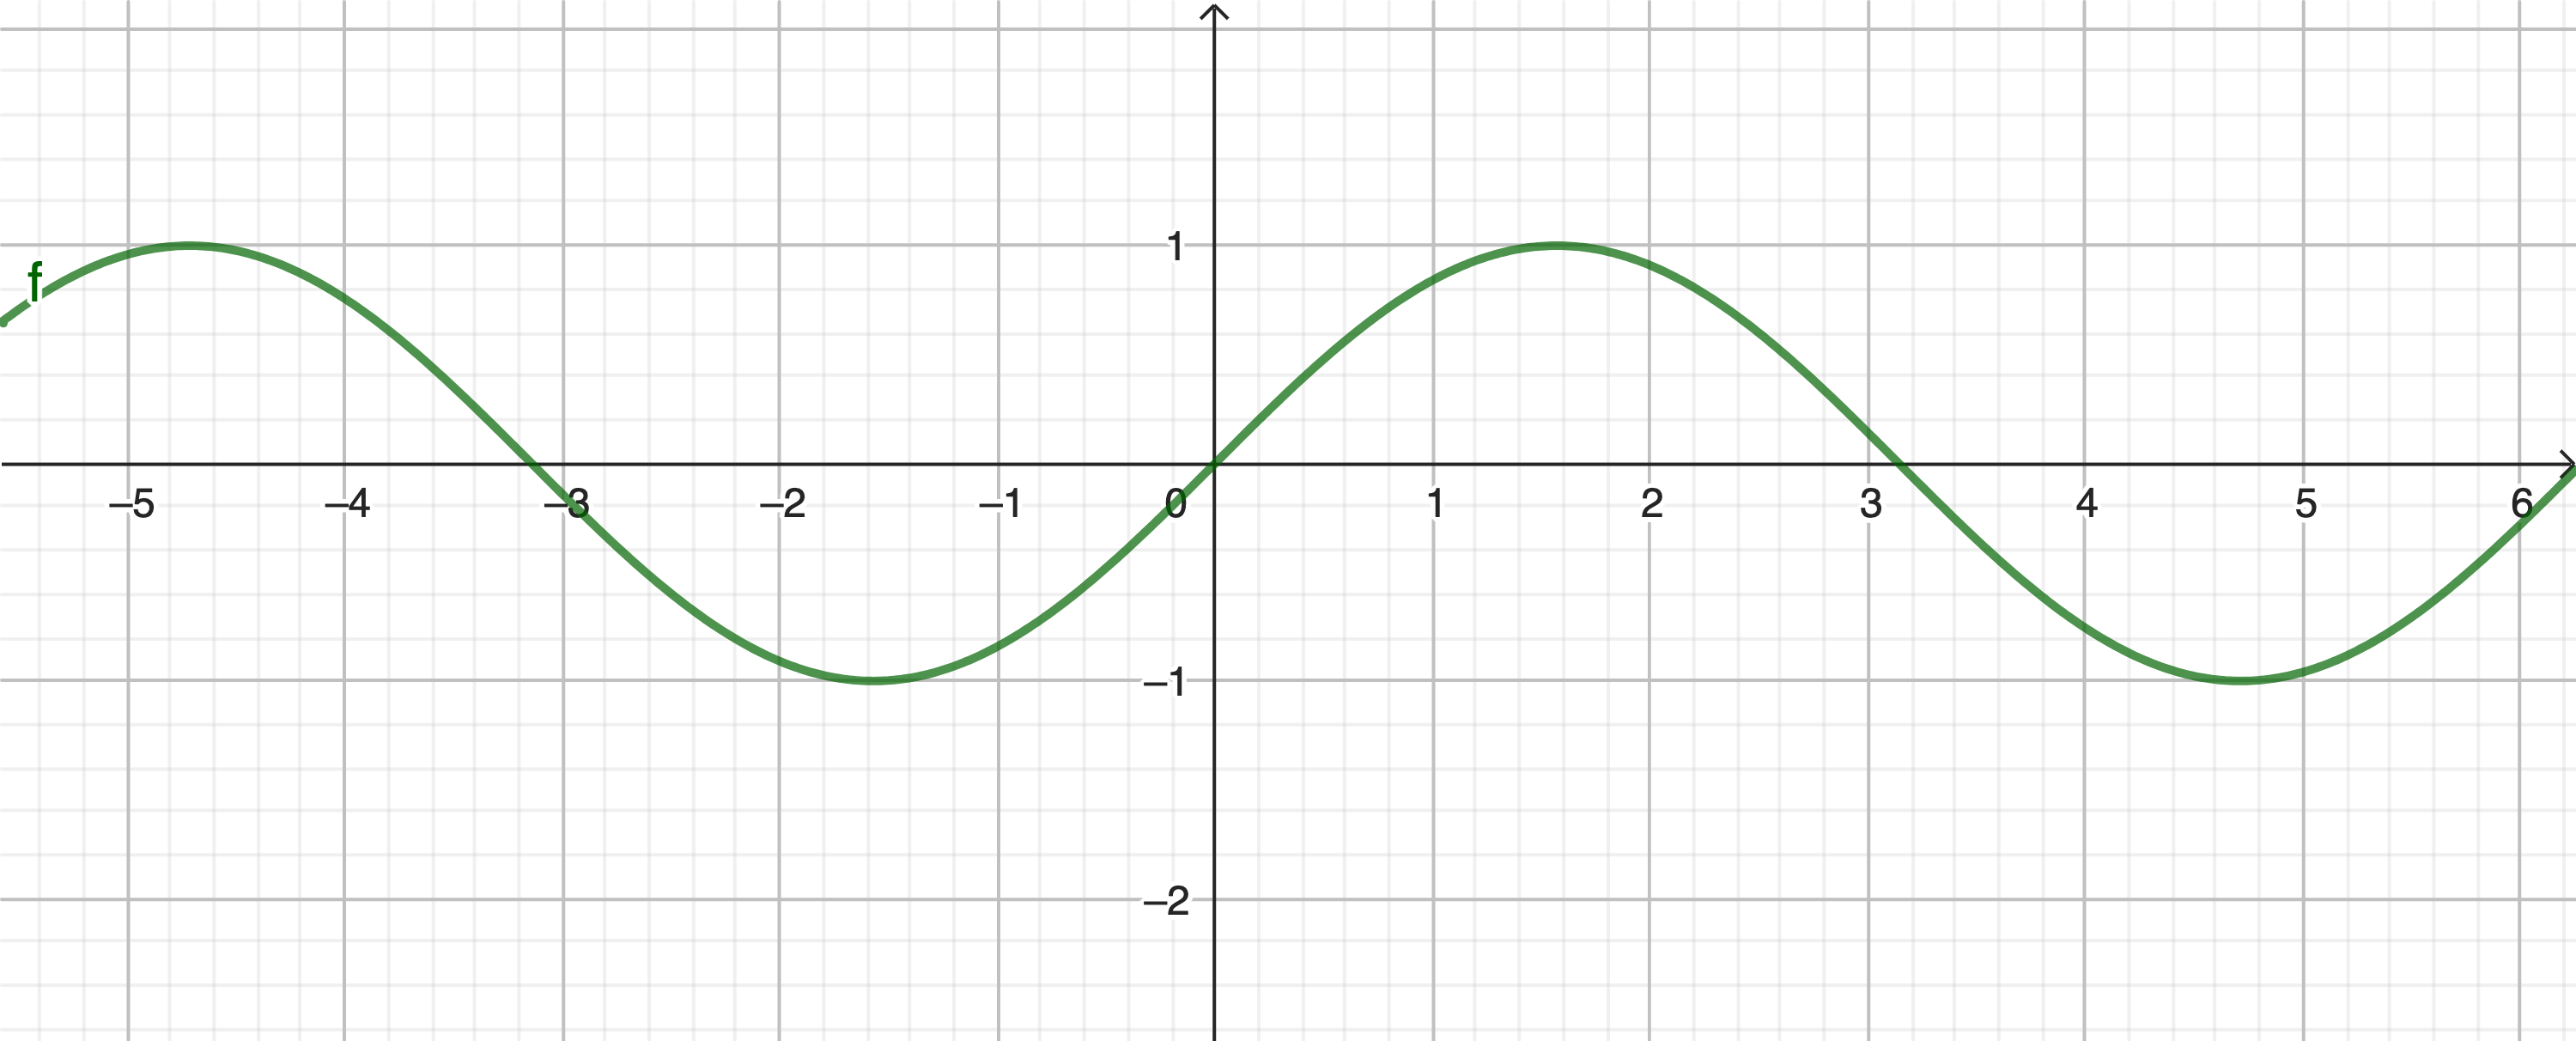
\includegraphics[width = 0.5 \textwidth]{media/IntroTaylor.png}
	\end{center}
	Ein Polynom ersten Grades ist eine lineare Funktion. Der Graph ist eine Gerade.

	Welche Gerade nähert sich um die Stelle $x_0=0$ am besten an den Graphen an?

	\vspace*{4cm}

	Approximation durch ein Polynom $T_2(x)$ 2. Grades:

	Ansatz: $T_2(x)=a_2x^2+a_1x+a_0$
	\vspace*{6cm}


\end{bsp}
\clearpage
\begin{LA}
	{Approximation der Sinusfunktion}{TaylorSinus}
	\begin{enumerate}
		\item 	Bestimmen Sie Näherungen der Funktion $f(x)=\sin(x)$ durch Polynome $T_3,T_4$ und $T_5$ vom Grad 3, 4 und 5 nach dem besprochenen Muster. Testen Sie jeweils die Genauigkeit an der Stelle $x=0.5$ (rad), indem Sie $\sin(0.5)$ mit $T_k (0.5)$ vergleichen.
		\item Können Sie die Polynome $T_6$ und $T_7$ angeben, ohne die ganze Rechnung erneut durchzuführen?
		\item Sei nun $f$ eine beliebige Funktion. 	Bestimmen Sie Polynomfunktionen $T_1,T_2$ und $T_3$ ersten, zweiten bzw. dritten Grades, die mit $f$ an der Stelle $x_0=0$ im Funktionswert und im Wert der 1., 2. und 3. Ableitung übereinstimmen.
		\item 	Wie lauten das Näherungspolynom $n$-ten Grades $T_n (x)$ für eine beliebige Funktion $f$?
	\end{enumerate}
\end{LA}

\clearpage


